\documentclass[10pt,border=5pt]{standalone}
\usepackage[T1]{fontenc}
\usepackage{lmodern,amsmath,amssymb,mathrsfs,tikz}
\usetikzlibrary{arrows.meta,positioning,calc}
\definecolor{ink}{HTML}{192536}
\definecolor{blue}{HTML}{2E70AE}
\definecolor{gold}{HTML}{A66A15}
\definecolor{green}{HTML}{28764D}
\definecolor{red}{HTML}{B43D3D}
\newcommand{\C}{\mathbb C}
\newcommand{\R}{\mathcal R}
\newcommand{\Lr}{\mathcal L_{\mathrm{res}}}
\newcommand{\Prs}{\mathcal P_{\mathrm{res}}}
\newcommand{\Tr}{T_{\mathrm{resp}}}
\newcommand{\rr}{\rho_{\mathrm{res}}}
\tikzset{every node/.style={font=\small,text=ink,align=center},
 box/.style={draw=blue,fill=blue!4,rounded corners=3pt,line width=.7pt,inner sep=7pt},
 goldbox/.style={box,draw=gold,fill=gold!5},
 greenbox/.style={box,draw=green,fill=green!5},
 redbox/.style={box,draw=red,fill=red!4},
 edge/.style={-{Stealth[length=4pt]},draw=ink,line width=.7pt},
 heading/.style={font=\small\bfseries},
 note/.style={font=\small,text=ink!85}}

\begin{document}
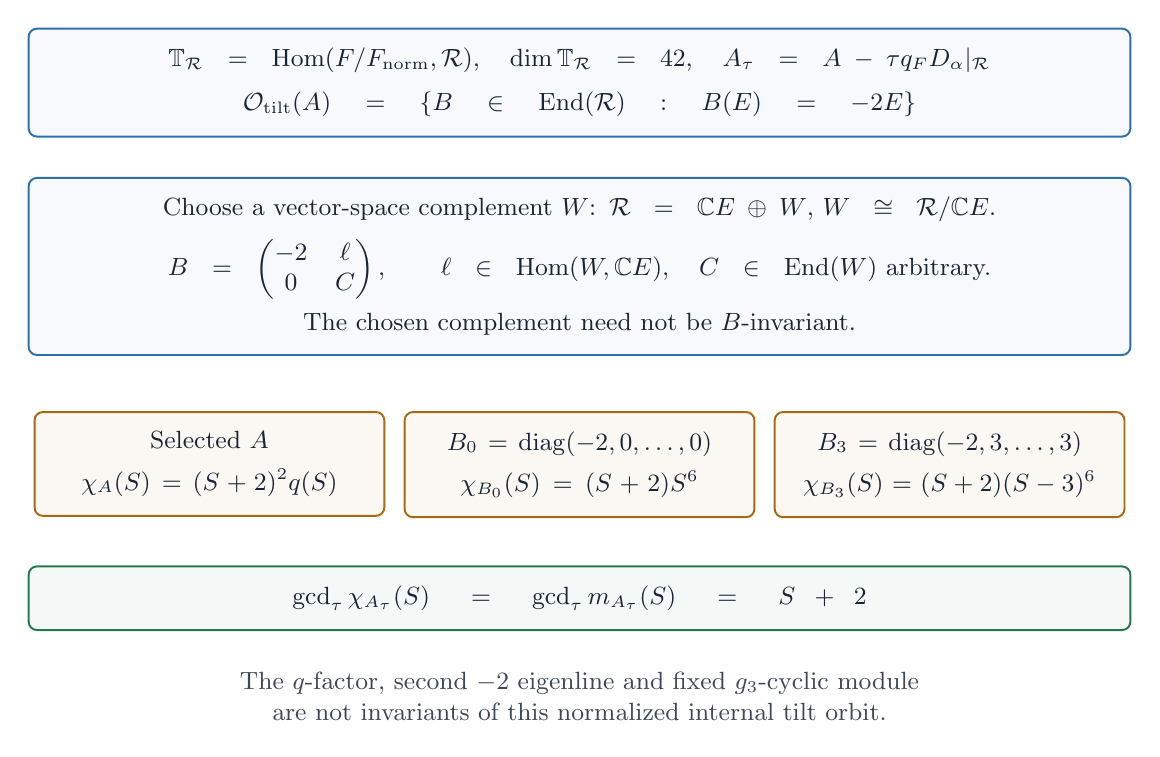
\begin{tikzpicture}
\node[box,text width=13.5cm] (orbit)
 {$\mathbb T_{\R}=\operatorname{Hom}(F/F_{\mathrm{norm}},\R),\quad
 \dim\mathbb T_{\R}=42,\quad A_\tau=A-\tau q_FD_\alpha|_{\R}$\\[5pt]
 $\mathcal O_{\mathrm{tilt}}(A)=\{B\in\operatorname{End}(\R):B(E)=-2E\}$};
\node[box,text width=13.5cm,below=5mm of orbit] (block)
 {Choose a vector-space complement $W$: $\R=\C E\oplus W$,
 $W\cong\R/\C E$.\\[5pt]
 $B=\begin{pmatrix}-2&\ell\\0&C\end{pmatrix},\qquad
 \ell\in\operatorname{Hom}(W,\C E),\quad C\in\operatorname{End}(W)$ arbitrary.\\[4pt]
 The chosen complement need not be $B$-invariant.};
\node[goldbox,text width=3.95cm,anchor=north] (a) at ($(block.south)+(-4.7,-.7)$)
 {Selected $A$\\[4pt]$\chi_A(S)=(S+2)^2q(S)$};
\node[goldbox,text width=3.95cm,below=7mm of block] (b0)
 {$B_0=\operatorname{diag}(-2,0,\ldots,0)$\\[4pt]
 $\chi_{B_0}(S)=(S+2)S^6$};
\node[goldbox,text width=3.95cm,anchor=north] (b3) at ($(block.south)+(4.7,-.7)$)
 {$B_3=\operatorname{diag}(-2,3,\ldots,3)$\\[4pt]
 $\chi_{B_3}(S)=(S+2)(S-3)^6$};
\node[greenbox,text width=13.5cm,below=6mm of b0] (gcd)
 {$\gcd_\tau\chi_{A_\tau}(S)=\gcd_\tau m_{A_\tau}(S)=S+2$};
\node[note,text width=13.5cm,below=4mm of gcd]
 {The $q$-factor, second $-2$ eigenline and fixed $g_3$-cyclic module\\
 are not invariants of this normalized internal tilt orbit.};
\end{tikzpicture}
\end{document}
